\section{Maximum Length Sequence(m-sequences)}

M-sequences are a binary pseudonoise construction that was initially conceived using
linear feedback shift registers (LFSR). A m-sequence is a binary sequence generated
by an LFSR that, given an initial state different from 0, it cycles between all
posible states except 0. (See Appendix for formal details) The following properties
hold for a m-sequences.

\begin{figure}
  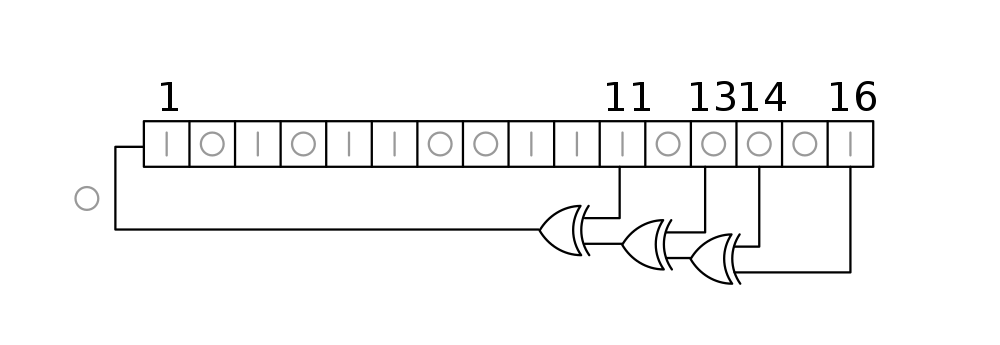
\includegraphics[scale=0.5]{Chapters/PRN_generation/LFSR-F16.svg.png}
  \caption{A diagram of a LFSR. The next symbol to be set in the register 1
  is computed based on the previous state. The previous registers are moved one
  to the right, discarding the last register.}
  \label{}
\end{figure}

\begin{itemize}
\item   A m-sequence will always be of length of the form $2^{m}-1$ where $m$ is an
  arbitrary natural number.
\item A m-sequence sequence will always have an autocorrelation function such as
  all the components will be -1 except when $\tau = 0$
\end{itemize}
The complexity of the algorithm to construct an m-sequence of length $n$ is $O(n)$.
However, the problem is that sequences of arbitrary length might be needed in some
applications.\\

 As it will be discussed in a following chapter, the complexity of computing the
autocorrelation with the Fourier Transform approach is $O(n \cdot log(n))$ so using longer length than the strictly needed  has a  negative direct practical consequences.\\

These sequences by themselves might not a be huge deal because they do not define a way to build families of sequences with low cross correlation, but they are the
building blocks for other constructions, such as the Gold Codes that are used in GPS and  CDMA.
